\scanpage{17}

% l. 1
\mspage{\textcircled{\scriptsize 13 bis}}
$S$ graphe \inserted{$\ne\varnothing$} tel que \deleted{l'ens de ses \unsure{arêtes est} \illegible{2} et}

% ll. 2–3
\[
\begin{aligned}
\text{a)}\quad&\forall x,y\in S\text{ liés},\quad\exists!z\in S\text{ tel que }z\text{ soit lié à }x\text{ et }y\\
\text{b)}\quad&\exists\,\nu\in\mathbb N^*\text{ tel que }\forall s\in S,\quad\operatorname{Card}\underbrace{E(s)}_{\{t\in S\mid t\text{ lié à }s\}}=\nu
\end{aligned}
\]

% ll. 4–6
\deleted{c)} \uline{Lemme 1} \inserted{$\nu$ est pair, et} On a $\operatorname{card} S\geq3(\nu-1)$. On a égalité \unsure{sss|ssi} $\forall$ \inserted{(\unsure{resp.|ou|il en} $\exists$)} triangle $T=\{x,y,z\}$ de $S$, \deleted{\unsure{à|a}} tt élément de $S^{\unsure{\prime|*}}=S-T$ est lié à un (et un seul) élément de $T$.

% ll. 7–10
\[
\begin{aligned}
\nu&=2(\mu+1)&2\\
\operatorname{card}S&=3(2\mu+1)&\operatorname{card} S-\operatorname{card}(E(s))\inserted{-1}&=\operatorname{card}(S-E(s)\inserted{-\{s\}})=4\mu\deleted{\unsure{+1}}\\
&&4\mu&\leq2^{\mu+1}\qquad\mu\leq2^{\mu-1}\\
&&&\deleted{\unsure{2\mu+1}}
\end{aligned}
\]

% left below computation, small triangle
\figure{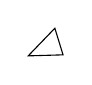
\begin{tikzpicture}[scale=.65]\draw (0,0)--(.52,.54)--(.68,.02)--cycle;\end{tikzpicture}}

% next to small triangle, looped graph
\figure{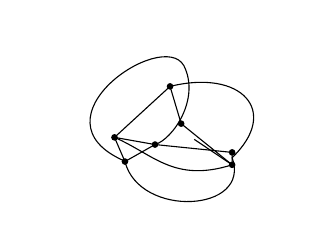
\begin{tikzpicture}[scale=.83]
\draw (0,0)--(.85,.78)--(1.02,.21)--(1.8,-.42)--(1.8,-.23)--(.62,-.11)--cycle;
\draw (.85,.78)..controls (1.95,1.05) and (2.54,.40)..(1.8,-.31) ..controls (2.10,-1.15) and (.38,-1.24)..(.16,-.37)--(0,0);
\draw (.15,-.36)..controls (-1.32,.28) and (.73,1.67)..(1.06,1.10)..controls (1.32,.59) and (.89,-.03)..(.62,-.11)--(.16,-.37);
\draw (0,0)..controls (.60,-.26) and (.91,-.70)..(1.8,-.42) (1.22,-.03)--(1.8,-.42);
\foreach \x/\y in {0/0,.85/.78,1.02/.21,.62/-.11,.16/-.37,1.8/-.42,1.8/-.23}{\fill (\x,\y) circle (1.45pt);}
\end{tikzpicture}}

% lower of three drawings, before fold
\figure{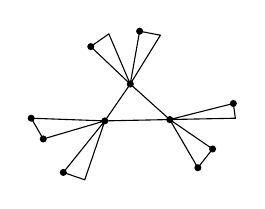
\begin{tikzpicture}[scale=.85]
\draw (0,0)--(.38,.55)--(.97,.02)--cycle;
\draw (0,0)--(-1.10,.04)--(-.92,-.27)--cycle (0,0)--(-.62,-.77)--(-.30,-.88)--cycle;
\draw (.38,.55)--(-.21,1.11)--(.06,1.30)--cycle (.38,.55)--(.52,1.34)--(.83,1.28)--cycle;
\draw (.97,.02)--(1.92,.26)--(1.95,.04)--cycle (.97,.02)--(1.61,-.42)--(1.39,-.70)--cycle;
\foreach \x/\y in {0/0,.38/.55,.97/.02,-1.1/.04,-.92/-.27,-.62/-.77,-.21/1.11,.52/1.34,1.92/.26,1.61/-.42,1.39/-.70}{\fill (\x,\y) circle (1.5pt);}
\end{tikzpicture}}
% archive sheet number: 16
